\documentclass{beamer}
\usepackage{beamerthemesplit}
\usepackage{wrapfig}
\usetheme{SPbGU}
\usepackage{pdfpages}
\usepackage{amsmath}
\usepackage{cmap} 
\usepackage[T2A]{fontenc} 
\usepackage[utf8]{inputenc}
\usepackage[english,russian]{babel}
\usepackage{indentfirst}
\usepackage{amsmath}
\usepackage{tikz}
\usepackage{multirow}
\usepackage[noend]{algpseudocode}
\usepackage{algorithm}
\usepackage{algorithmicx}
\usetikzlibrary{shapes,arrows}
\usepackage{fancyvrb}
\newtheorem{rutheorem}{Теорема}
\newtheorem{ruproof}{Доказательство}
\newtheorem{rudefinition}{Определение}
\newtheorem{rulemma}{Лемма}
\beamertemplatenavigationsymbolsempty

\title[]{Реализация алгоритма поиска путей с контекстно-свободными ограничениями для графовой
базы данных Neo4j}
% То, что в квадратных скобках, отображается в левом нижнем углу. 
\institute[СПбГУ]{
Санкт-Петербургский государственный университет \\
Кафедра системного программирования }

% То, что в квадратных скобках, отображается в левом нижнем углу.
\author[Погожельская Влада]{Погожельская Влада Владимировна, 18.Б11-мм \\
  % У научного руководителя должна быть указана научная степень
  \and  
    {\bfseries Научный руководитель:} к.\,ф.-м.\,н., доцент Григорьев С.\,В. \\ 
  % Для курсовой не обязателен. Должна быть указана должность или ученая степень
}
\date{06 июня 2020г.}

\definecolor{orange}{RGB}{179,36,31}

\begin{document}
{
% Лого университета или организации, отображается в шапке титульного листа
\begin{frame}
  \begin{center}
  {
\includegraphics[width=1.5cm]{pictures/SPbGU_Logo.png}}
  \end{center}
  \titlepage
\end{frame}
}

\begin{frame}[fragile]
  \transwipe[direction=90]
  \frametitle{Введение}
  \begin{itemize}
    \item \textbf{Подсчет количества треугольников в графе} --- количество уникальных троек вершин $u, v, w$ в неориентированном графе: $(u, v), (u, w), (v, w) \in E$, где $E$ --- множество ребер графа
    \item \textbf{Область применения}: анализ социальных сетей (обнаружение сообществ и степени сплоченности между ними, коэффициент кластеризации и транзитивности)
    \item Для решения задачи применяются методы линейной алгебры
  \end{itemize}
\end{frame}

\begin{frame}
  \transwipe[direction=90]
  \frametitle{Цели и задачи}
  \textbf{Целью} данной работы является сравнительный анализ существующих на данный момент решений задачи подсчета количества треугольников, основанных на линейной алгебре
  
  \textbf{Задачи}:
  \begin{itemize}
    \item Выполнить обзор существующих решений задачи о подсчете количества треугольников, основанных на линейной алгебре
    \item Выполнить реализацию выбранного в результате обзора алгоритма подсчета количества треугольников в графе с помощью выбранной библиотеки
    \item Провести экспериментальное исследование реализованного алгоритма и уже существующих в выбранной библиотеке
  \end{itemize}
\end{frame}

\begin{frame}
  \transwipe[direction=90]
  \frametitle{Обзор существующих решений}
  \begin{itemize}
      \item $A$ --- матрица смежности входного графа
      \item $U$ --- верхнетреугольная, $L$ --- нижнетреугольная: A = L + U
      \item (*) --- умножение матриц, (.*) --- поэлементное умножение, (') --- транспонирование
  \end{itemize}
  \textbf{Алгоритмы}
  \begin{itemize}
    \item \textbf{Базовая версия матричного алгоритма} --- $ntri = \frac{1}{6}trace(A^{3})$
    \item \textbf{Burkhardt algorithm} --- $ntri = \frac{1}{6} sum (sum ((A^{2}) .* A))$
    \item \textbf{Cohen algorithm} --- $ntri = \frac{1}{2}\sum\limits_j (\sum\limits_i ((L * U) .* A))$
    \item \textbf{Sandia algorithm} --- $ntri = \sum\limits_j (\sum\limits_i ((U * U) .* U))$
    \item \textbf{SandiaDot algorithm} --- $ntri = \sum\limits_j (\sum\limits_i ((L * U') .* L))$
  \end{itemize}
  \end{frame}
  
\begin{frame}
  \transwipe[direction=90]
  \frametitle{Обзор существующих решений}
  \textbf{Библиотеки}\\
  GraphBLAS ---  стандарт для разработки графовых алгоритмов в терминах линейной алгебры
  \begin{itemize}
    \item \textbf{GraphBLAS Template Library (GBTL)} --- реализация GraphBLAS для языка C++, поддерживающая реализация алгоритма Cohen
    \item \textbf{GraphBLAST} --- реализация GraphBLAS для GPU, алгоритм не может быть реализован
    \item \textbf{SuiteSparse:GraphBLAS} --- одна из самых полных реализаций стандарта, содержащая все вышеописанные алгоритмы подсчета количества треугольников, кроме базового
  \end{itemize}
  \end{frame}
  
\begin{frame}
  \transwipe[direction=90]
    \frametitle{Выводы из обзора}
    \begin{itemize}
      \item Вопрос о практической применимости базового алгоритма не исследован до конца
      \item В качестве библиотеки для реализации был выбран SuiteSparse
    \end{itemize}
\end{frame}

\begin{frame}
  \transwipe[direction=90]
  \frametitle{Алгоритм}
  Дан неорграф $G = (V, E)$, $A$ --- матрица смежности размера $N \times N$ \\ 
  \begin{itemize}
      \item $A^n[i][j]$ --- количество различных путей в графе из $i$ в $j$ длины n
      \item $A^3[i][i]$ --- количество треугольников, проходящих через вершину $i$
      \item Число треугольников в графе : $\frac{1}{6} trace(A^{3})$
  \end{itemize}
\end{frame}

\begin{frame}
  \transwipe[direction=90]
  \frametitle{Особенности реализации с помощью SuiteSparse:GraphBLAS}
  \begin{itemize}
      \item Функция перемножения двух разреженных матриц $GrB\_mxm$ использует полукольцо
      \item В SuiteSparse скалярное сложение в стандартном умножении матриц заменяется моноидом
      \item Полукольцо ($GrB\_Semiring$) состоит из моноида и оператора «умножения», вместе эти операции определяют операцию матричного умножения
      \item В данной реализации был использован оптимизированный метод умножения матриц --- Gustavson's method
  \end{itemize}
\end{frame}

\begin{frame}
  \transwipe[direction=90]
  \frametitle{Архитектура решения}
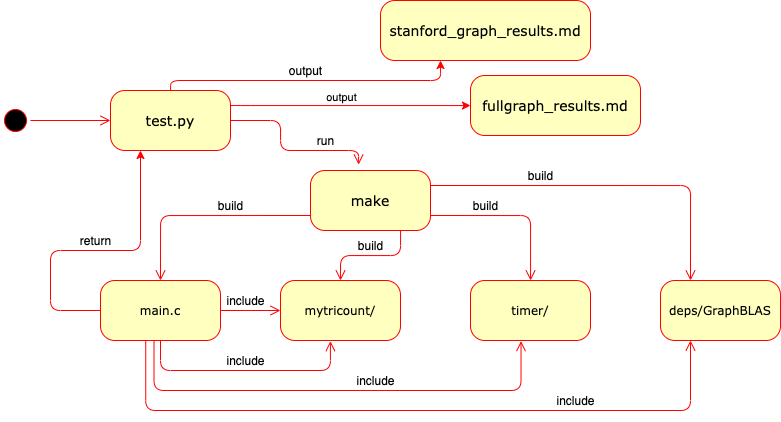
\includegraphics[width=12cm]{./pictures/arch1.png}
\end{frame}

\begin{frame}
  \transwipe[direction=90]
  \frametitle{Cравнительный анализ}
  \capture{Результаты замеров на полных графах, время указано в секундах}
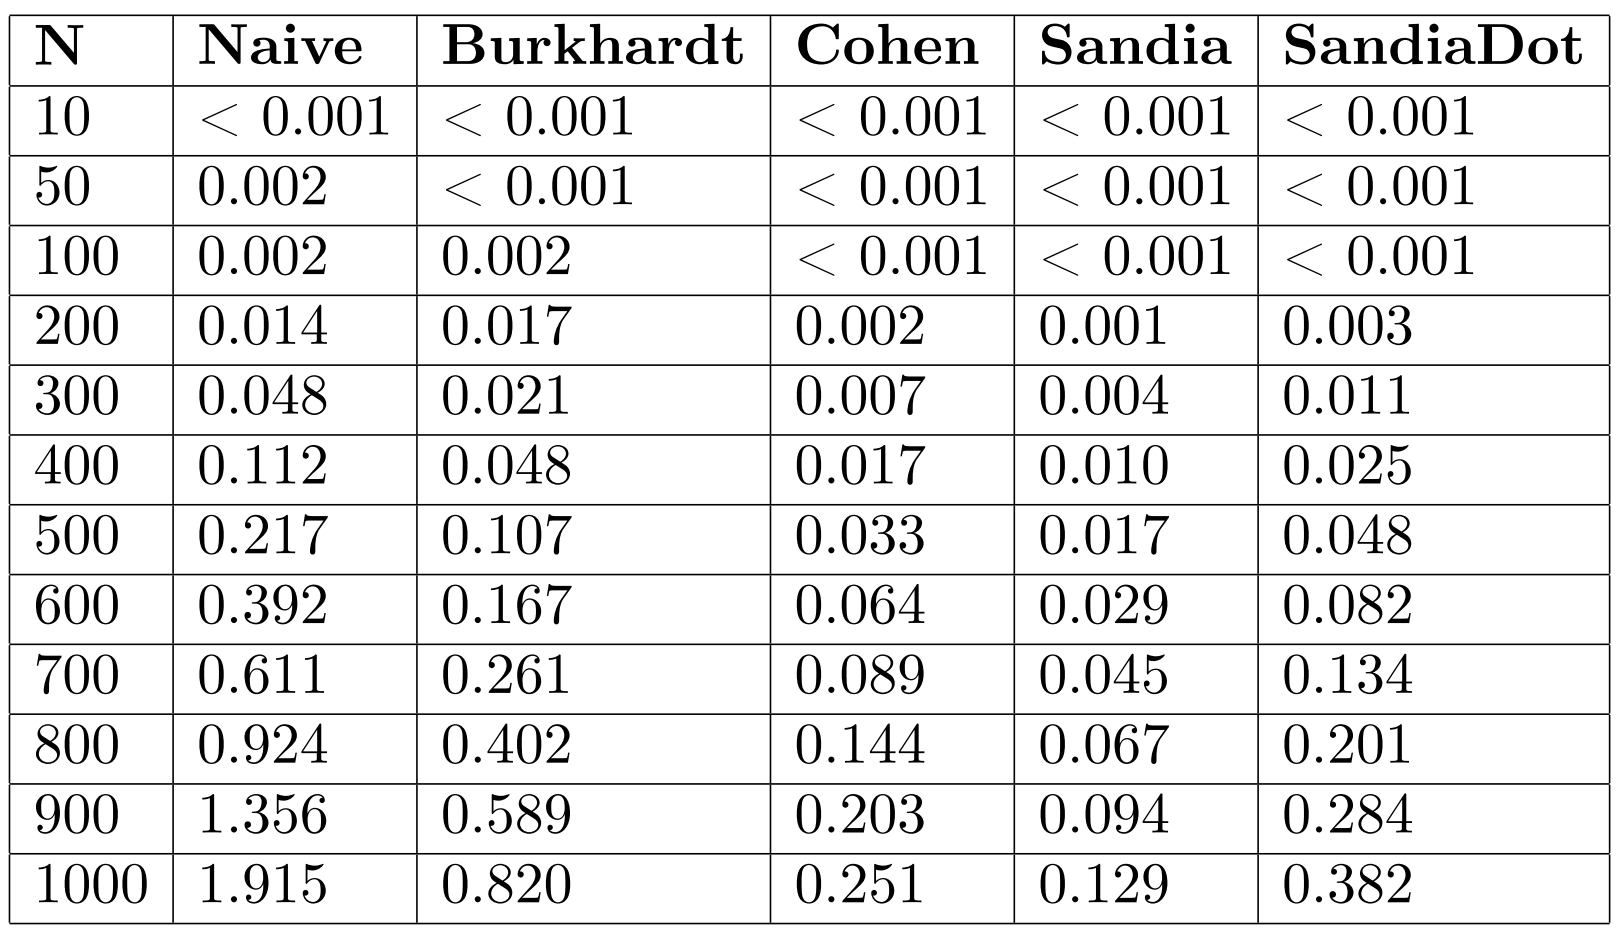
\includegraphics[width=12cm]{./pictures/t1.png}
\end{frame}

\begin{frame}
  \transwipe[direction=90]
  \frametitle{Cравнительный анализ}
  \capture{Результаты замеров на реальных графах, время указано в секундах}
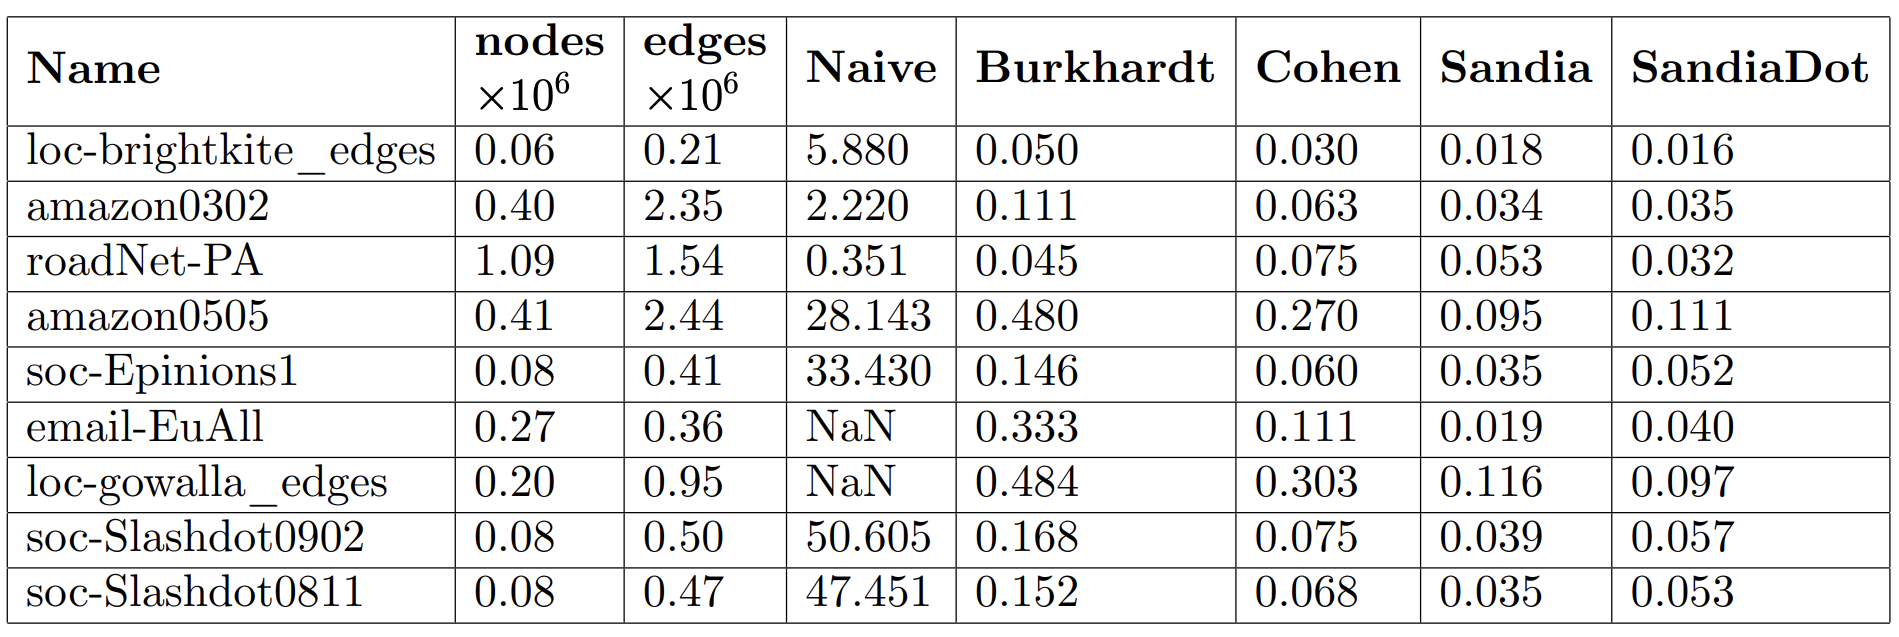
\includegraphics[width=12cm]{./pictures/t2.png}

\end{frame}

\begin{frame}
  \transwipe[direction=90]
  \frametitle{Результаты}
Были выполнены следующие задачи:
\begin{itemize}
    \item Выполнен обзор существующих решений задачи о подсчете количества треугольников, основанных на линейной алгебре, и использованных для этого инструментов
    \item Выполнена реализация выбранного алгоритма подсчета количества треугольников в графе с помощью библиотеки GraphBLAS: SuiteSparse
    \item Проведено экспериментальное исследование реализованного алгоритма и уже существующих в данной библиотеке
\end{itemize}
\end{frame}

\end{document}
